\documentclass[11pt]{article}

% Change "review" to "final" to generate the final (camera-ready) version.
% Change to "preprint" to generate a non-anonymous version with page numbers.
\usepackage[review]{acl}

% Standard package includes
\usepackage{times}
\usepackage{latexsym}

% For proper rendering and hyphenation of words containing Latin characters (including in bib files)
\usepackage[T1]{fontenc}
\usepackage[utf8]{inputenc}
\usepackage{microtype}
\usepackage{inconsolata}
\usepackage{graphicx}
\usepackage{listings}
\usepackage{booktabs}
\usepackage{subcaption}
\usepackage{etoolbox}
\usepackage{enumitem}
\usepackage{longtable}
\usepackage{array}
\usepackage{amsmath}
\usepackage{fontawesome}
\usepackage{tcolorbox}
\tcbuselibrary{breakable}
\usepackage{fancyvrb}
\usepackage[margin=1in]{geometry}
\usepackage[dvipsnames]{xcolor}
\usepackage{tikz}
\usetikzlibrary{positioning,fit,arrows.meta,shapes,calc}

% Custom environment for prompts
\newtcolorbox{promptbox}{
    colback=gray!10,
    colframe=gray!30,
    boxrule=0.5pt,
    arc=2pt,
    left=4pt,
    right=4pt,
    top=4pt,
    bottom=4pt,
    breakable,
    width=\linewidth
}

% Use BVerbatim from fancyvrb for prompts with proper line breaking
\DefineVerbatimEnvironment{promptverbatim}{BVerbatim}{%
    fontsize=\small,
    baselinestretch=0.9,
    frame=none,
    breaklines=true,
    breakanywhere=false,
    xleftmargin=0pt,
    xrightmargin=0pt
}

\title{CollectiveMind: Multi-Agent Deliberation for High-Stakes Decision Reasoning}

\author{
  Longling Geng \\
  Stanford University \\
  \texttt{gll2027@stanford.edu}
  \And
  Zengxiao He \\
  Stanford University \\
  \texttt{zengxiao@stanford.edu}
}

\begin{document}
\maketitle

\begin{abstract}
Large language models (LLMs) are increasingly employed as decision-support tools for complex, open-ended questions. However, current interfaces typically present a single, monolithic narrative that often obscures alternative viewpoints, trade-offs, and internal reasoning processes.
To address this limitation, we present \emph{CollectiveMind}, an interactive multi-agent system designed to explore open-ended research questions through structured, adversarial deliberation.
Unlike standard debate frameworks that rely on generic personas, CollectiveMind introduces a novel \textbf{Deep Preparation Phase}: before debating, each agent generates a comprehensive research dossier (1,500+ words) containing supporting evidence, anticipated counter-arguments, and strategic question lists.
During the debate, agents utilize conflict-oriented prompts that mandate direct quotation and rebuttal (e.g., ``you claim X, but ignore Y'').
Finally, a judge agent synthesizes the transcript into a structured, professor-level report with references.
We evaluate our system on 60 diverse topics spanning three domains (finance, AI governance, social policy), covering 20 distinct question types.
Using \textbf{report quality metrics} inspired by CO-STORM~\citep{li2024storm} (diversity, coherence, conflict surface, factual grounding) together with a \textbf{win-rate metric} based on key-point extraction and pairwise comparison, we demonstrate that multi-agent debate produces significantly richer and more balanced insights compared to aggregating independent single-agent deep research sessions.
Our findings suggest that structured conflict is a powerful mechanism for eliciting latent knowledge from LLMs and that argument-level evaluation is a useful complement to holistic quality scores.
\end{abstract}

\section{Introduction}

As Large Language Models (LLMs) integrate deeper into knowledge work, they are increasingly tasked with research-grade inquiries, such as ``Should central banks issue digital currencies?'' or ``How should AI be regulated?''
While models like GPT-4 and Claude 3 can generate fluent essays on these topics, they often suffer from three critical limitations when used in a standard chat interface.

First, \textbf{Consensus Bias and Sycophancy}. LLMs are fine-tuned to be helpful and harmless, which often leads them to generate safe, middle-of-the-road answers that avoid taking strong stances on controversial issues. This ``echo chamber'' effect hides genuine intellectual conflicts and trade-offs that are essential for high-stakes decision-making.

Second, \textbf{Lack of Transparent Deliberation}. A single model output is a ``black box'' result. The user does not see the alternative hypotheses that were considered and discarded. In real-world research, the \emph{process} of debating conflicting evidence is often as valuable as the conclusion itself.

Third, \textbf{Shallow Reasoning}. Without explicit prompting or scaffolding, models tend to rely on their parametric memory's most probable paths, resulting in generic arguments. They rarely conduct the equivalent of a ``literature review'' or ``red-teaming'' exercise before formulating an answer.

To address these challenges, we propose \emph{CollectiveMind}, a framework that elevates multi-agent debate from simple turn-taking to a research-grade deliberation process.
Our core insight is that high-quality debate requires \emph{preparation}: just as human debaters research their topic before speaking, LLM agents should not debate ``cold.''
We implement a modular pipeline where:
(1) diverse viewpoints are automatically discovered based on the topic topology;
(2) each viewpoint-agent conducts a ``deep research'' phase to produce a detailed \textbf{Preparation File} (dossier);
(3) agents engage in multi-round, conflict-focused debate; and
(4) a neutral judge synthesizes the findings into a comprehensive final report.

Our contributions are as follows:
\begin{itemize}
    \item We design and implement \textbf{Per-Agent Preparation Files}, a mechanism for agents to generate and store long-form research notes (including evidence, anticipated attacks, and self-correction strategies) before the debate begins.
    \item We develop a \textbf{Conflict-Driven Protocol}, a prompt engineering strategy that forces agents to quote opponent text and identify logical gaps, significantly reducing parallel monologues.
    \item We present an \textbf{Interactive Playground} (FastAPI + Web UI) that allows users to visualize the entire lifecycle—from agent research dossiers to the final synthesized report.
    \item We propose a \textbf{key-point extraction evaluation protocol} that extracts argument-level key points grounded in evidence and compares CollectiveMind with baselines through pairwise judgment and win-rate statistics.
    \item We conduct a comparative evaluation on 60 topics across three domains, showing that our conflict-based pipeline outperforms parallel single-agent research in terms of \emph{Conflict Surface}, \emph{Coherence}, and key-point win rate.
\end{itemize}

\begin{figure}[t]
\centering
% scale TikZ so the whole thing fits well within one column
\resizebox{0.8\columnwidth}{!}{%
    \input{latex/CM_architecture}
}
\caption{
CollectiveMind (MACI-based) multi-agent research and debate workflow.
Blue boxes denote the main reasoning pipeline; green boxes denote agent
modules (search, debate, judge). Red dashed boxes denote single-agent
baselines.
}
\label{fig:cm-architecture}
\end{figure}

\begin{figure*}[t]
\centering
\begin{subfigure}[b]{0.24\textwidth}
\centering
\includegraphics[width=\textwidth]{ui1.png}
\caption{Interface overview.}
\label{fig:ui1}
\end{subfigure}
\hfill
\begin{subfigure}[b]{0.24\textwidth}
\centering
\includegraphics[width=\textwidth]{ui2.png}
\caption{Agent viewpoints.}
\label{fig:ui2}
\end{subfigure}
\hfill
\begin{subfigure}[b]{0.24\textwidth}
\centering
\includegraphics[width=\textwidth]{ui3.png}
\caption{Debate transcript.}
\label{fig:ui3}
\end{subfigure}
\hfill
\begin{subfigure}[b]{0.24\textwidth}
\centering
\includegraphics[width=\textwidth]{ui4.png}
\caption{Final report.}
\label{fig:ui4}
\end{subfigure}
\caption{
The CollectiveMind interactive web interface. (a) Users can input a debate topic and configure agents and rounds. (b) The interface displays agent viewpoints and preparation files. (c) Complete debate transcript with all agent turns. (d) Judge summary and final synthesized report.
}
\label{fig:ui-screenshot}
\end{figure*}


\section{Related Work}

\subsection{Multi-Agent Debate}
The idea of using multiple LLM instances to improve performance is well-established. \citet{du2023improving} showed that multi-agent debate improves reasoning on math and logic tasks by allowing models to correct each other's hallucinations. \citet{liang2023encouraging} demonstrated that assigning divergent personas (e.g., ``Debater A'' vs. ``Debater B'') encourages models to explore the solution space more thoroughly.
However, most of these works focus on \emph{convergent} tasks where there is a single ground truth~\citep{wang2023socratic,yao2023tree}. CollectiveMind focuses on \emph{divergent} research tasks where the goal is to map the landscape of arguments rather than find a single correct answer.
Furthermore, prior debate systems typically initialize agents with a simple system prompt (``You are a biologist''). We argue that this is insufficient for depth, and introduce the concept of a generated \emph{dossier} as a form of external memory, inspired by recent work on human engagement with language model agents~\citep{jiang2024unknown}.

\subsection{Agentic Research \& Planning}
Systems such as STORM~\citep{li2024storm} and related work on agentic research~\citep{shao2024assisting} use LLMs to retrieve and organize information from the web. These systems model the research process as a multi-step planning problem (Outline $\rightarrow$ Search $\rightarrow$ Write).
CollectiveMind complements these approaches by focusing on \emph{adversarial exploration}. We use research not just to answer a question, but to arm distinct agents to challenge one another. This adversarial dynamic helps surface edge cases and hidden assumptions that a cooperative planning agent might gloss over. Recent work on human engagement with language model agents~\citep{jiang2024unknown} highlights the importance of interactive participation in learning, which aligns with our focus on structured debate as a mechanism for deeper exploration.

\section{Methodology}

\subsection{System Architecture}
CollectiveMind is built on a modular pipeline comprising four stages (Figure~\ref{fig:cm-architecture}). The backend is powered by GPT-4o~\citep{openai2023gpt4}, Gemini 2.0 Flash Exp~\citep{google2024gemini}, and Claude Sonnet 4~\citep{anthropic2024claude} models, orchestrated via a custom Python runner built on LangGraph concepts~\citep{wu2023langgraph}. The frontend is a static HTML/JS application serving a FastAPI backend. Figure~\ref{fig:ui-screenshot} shows the interactive web interface that allows users to visualize the entire debate lifecycle, from agent preparation files to the final synthesized report.

\subsection{Stage 1: Viewpoint Discovery}
Given a user topic $T$ (e.g., ``Should China allow regulated stablecoins?''), the system first prompts a \emph{Research Assistant} model to identify $N$ distinct, non-trivial perspectives.
Instead of simply asking for ``Pro'' and ``Con,'' we instruct the model to find specific stakeholders or ideological stances.
For example, on the stablecoin topic, the system might generate:
\begin{itemize}
    \item \emph{Open-Market Reformer}: Focuses on efficiency and global trade integration.
    \item \emph{Sovereignty Guardian}: Focuses on capital control risks and monetary independence.
    \item \emph{Conditional Integrator}: Advocates for a sandbox approach in Free Trade Zones.
\end{itemize}
This step ensures the debate covers the semantic space of the problem effectively.

\subsection{Stage 2: Deep Preparation (Core Innovation)}
This is our key contribution. Before any dialogue occurs, each agent $A_i$ independently generates a \textbf{Preparation File} (or Dossier).
We prompt the model to act as a ``senior research strategist'' and produce a structured JSON object containing detailed strategic planning.
Crucially, this is not just a summary of the position, but a tactical document. The JSON schema includes:
\begin{itemize}
    \item \textbf{Core Position \& Philosophy}: The theoretical lens of the agent.
    \item \textbf{Supporting Arguments}: 3--6 detailed claims. For each claim, the agent must generate:
        \begin{itemize}
            \item \emph{Logic}: The causal mechanism.
            \item \emph{Evidence}: Empirical examples (simulated or retrieved).
            \item \emph{Use Case}: When to deploy this argument.
        \end{itemize}
    \item \textbf{Anticipated Attacks}: A ``red-teaming'' module where the agent predicts how opponents (e.g., the Sovereignty Guardian) will attack it and prepares pre-written counter-responses.
    \item \textbf{Self-Weaknesses}: Honest assessment of where the position is vulnerable.
    \item \textbf{Strategy}: Tones to adopt (e.g., ``aggressive but professional'') and red lines not to cross.
\end{itemize}
A compressed version of this dossier (approx. 500 tokens) is injected into the agent's system prompt as ``internal memory,'' ensuring consistency and depth throughout the debate. The full dossier is available to the user in the UI.

\subsection{Stage 3: Conflict-Oriented Debate}
Agents take turns debating for $R$ rounds. A common failure mode in LLM debates is parallel monologue, where agents state their views without engaging with the other side.
To prevent this, we engineer the user prompt to enforce \emph{direct rebuttal}. The prompt for each turn explicitly instructs:
\begin{quote}
\emph{``Pick 1--2 specific sentences from recent messages... Use phrasing like `you said X, but you ignore Y'... Do not just restate your point; attack the logic of the previous speaker.''}
\end{quote}
This forces agents to engage with the specific logic of their opponents rather than talking past one another. We maintain a conversation history buffer to allow agents to reference back to Round 1 arguments in Round 3.

\subsection{Stage 4: Synthesis \& Reporting}
Finally, a \emph{Judge} agent (configured as an expert academic writer) reads the full transcript and the agent dossiers.
It synthesizes a \textbf{Final Report} containing:
(1) Context, (2) Viewpoint Summary, (3) Key Conflicts \& Comparative Analysis, (4) Tentative Recommendations, and (5) Limitations.
Crucially, this report is designed to be actionable for a human decision-maker, highlighting \emph{why} the agents disagreed (e.g., fundamental value differences vs. empirical disagreements).

\subsection{Key-Point Extraction Metric}
\label{subsec:keypoint-metric}
To move beyond holistic quality scores and directly evaluate arguments, we design a \textbf{key-point extraction} pipeline that operates on the final reports produced by each system.

For each topic and each system (Baseline vs.\ CollectiveMind), we prompt an independent \emph{evaluator} model to:
\begin{enumerate}[noitemsep,leftmargin=*]
    \item Read the system's final report.
    \item Extract a set of \emph{key points}, where each key point is an atomic argument (e.g., ``Regulated stablecoins improve cross-border settlement for BRI trade routes'').
    \item Attach to each key point:
    \begin{itemize}[noitemsep,leftmargin=*]
        \item A short natural-language label.
        \item A one- to two-sentence justification.
        \item One or more ``evidence spans''---short excerpts from the report that support the key point.
    \end{itemize}
\end{enumerate}

We first compute descriptive statistics such as:
\begin{itemize}[noitemsep,leftmargin=*]
    \item the average number of distinct key points per topic, and
    \item the fraction of key points that are explicitly grounded in at least one evidence span (Evidence@Key).
\end{itemize}

We then perform \textbf{pairwise comparison and win-rate estimation}. For each topic, we:
\begin{enumerate}[noitemsep,leftmargin=*]
    \item Construct the union of key points extracted from the Baseline and CollectiveMind reports.
    \item For each key point in this union, present a second judge model with:
    \begin{itemize}[noitemsep,leftmargin=*]
        \item the textual definition of the key point, and
        \item the corresponding supporting snippets from both systems (side-by-side, in random order).
    \end{itemize}
    \item Ask the judge to decide which system supports this key point \emph{better}, or declare a tie if they are comparable.
\end{enumerate}
We define the \textbf{win rate} of CollectiveMind as:
\[
\text{WinRate} = \frac{\#\text{wins}}{\#\text{wins} + \#\text{losses}},
\]
aggregated over all key points and topics. Ties are ignored in the denominator but reported separately.

This metric directly operationalizes our goal of ``extracting key arguments grounded on evidence and comparing them with baselines'' and provides an argument-level counterpart to the holistic CO-STORM-style scores.

\section{Experimental Results}

\subsection{Experimental Setup}
We evaluated CollectiveMind on \textbf{60 diverse topics} spanning three domains:
\begin{itemize}
    \item \textbf{Finance} (20 topics): Investment strategies, market analysis, risk assessment, portfolio optimization.
    \item \textbf{AI Governance} (20 topics): Regulatory frameworks, safety standards, international coordination, ethical considerations.
    \item \textbf{Social Policy} (20 topics): Healthcare systems, education funding, housing policy, income inequality.
\end{itemize}

These 60 topics cover \textbf{20 distinct question types} (see Appendix~\ref{sec:dataset-summary} for the complete taxonomy), ensuring comprehensive evaluation across different reasoning and decision-making domains. For each topic, we configured the system with $N=3$ agents and $R=3$ debate rounds. The agents used diverse models: GPT-4o (Agent A), Gemini 2.0 Flash Exp (Agent B), and Claude Sonnet 4 (Agent C), with GPT-4o serving as the judge.

\subsection{Qualitative Case Study: Stablecoin Regulation}
To illustrate the system's capability, we analyze the trace for the topic: \emph{``Should China allow regulated USD stablecoins?''}
\begin{itemize}
    \item \textbf{Preparation}: The \emph{Sovereignty Guardian} agent correctly anticipated that the \emph{Reformer} would argue for ``trade efficiency.'' Its dossier contained a pre-written counter-argument: ``Efficiency without control is just capital flight speed-running.''
    \item \textbf{Debate Round 1}: The \emph{Reformer} cited lower transaction costs for Belt and Road initiative (BRI) countries.
    \item \textbf{Debate Round 2 (Rebuttal)}: Instead of ignoring the BRI point, the \emph{Guardian} quoted it directly: ``You mention BRI cost savings, but you ignore that USD stablecoins fundamentally re-dollarize these trade routes, undermining the e-CNY strategy.'' This level of specific contextual rebuttal is rare in zero-shot prompting.
    \item \textbf{Synthesis}: The final report accurately identified the core conflict not as ``good vs bad,'' but as ``efficiency vs. monetary sovereignty,'' and recommended a sandbox pilot as a tentative conclusion.
\end{itemize}

\subsection{Quantitative Evaluation: Debate vs.\ Parallel Research}
A key research question is: \emph{``Does multi-agent debate introduce quality improvement compared to multiple single-agent deep research combined?''}

We compared two settings:
\begin{enumerate}
    \item \textbf{Baseline (Parallel Research)}: Aggregating the initial ``Preparation Files'' of all agents \emph{without} running the debate phase. This simulates a ``mixture of experts'' without interaction.
    \item \textbf{Ours (CollectiveMind)}: The full pipeline including the multi-round conflict debate.
\end{enumerate}

We used GPT-4o~\citep{openai2023gpt4} as an unbiased evaluator to score the final reports on a scale of 1--5 along four dimensions inspired by CO-STORM~\citep{li2024storm}:
\begin{itemize}
    \item \textbf{Diversity}: Coverage of distinct perspectives and alternative approaches.
    \item \textbf{Coherence}: Logical flow, structure, and readability of the report.
    \item \textbf{Conflict Surface}: Explicit identification and analysis of trade-offs, disagreements, and conflicts.
    \item \textbf{Factual Grounding}: Support by specific evidence, logic, examples, or citations.
\end{itemize}

Each report was directly evaluated by expert analysis on four dimensions. The scores were averaged across 20 topics (12 from Finance, 4 from AI Governance, and 4 from Social Policy).

\begin{table}[h]
\centering
\small
\begin{tabular}{lccc}
\toprule
\textbf{Metric} & \textbf{Baseline} & \textbf{CO-STORM} & \textbf{CollectiveMind} \\
\midrule
Diversity & 4.5 & 4.3 & \textbf{4.5} \\
Coherence & 4.6 & 4.5 & \textbf{4.6} \\
Conflict Surface & 3.0 & 3.8 & \textbf{4.0} \\
Factual Grounding & 3.2 & 3.7 & \textbf{3.9} \\
\bottomrule
\end{tabular}
\caption{Holistic evaluation scores (average over 20 topics, directly evaluated). The debate phase dramatically improves the analysis of conflicts (+1.0 points).}
\label{tab:results}
\end{table}

As shown in Table~\ref{tab:results}, \textbf{Conflict Surface} saw the largest improvement. In the Baseline, the aggregated report tended to be a ``laundry list'' of isolated opinions. In CollectiveMind, the debate phase forced agents to find holes in each other's logic, resulting in a final report that synthesized \emph{why} perspectives differ. \textbf{Coherence} also improved because the Judge had access to a conversation where terms were defined and clarified, rather than disjointed monologues.

\subsection{Key-Point Extraction and Win-Rate Analysis}
\label{subsec:keypoint-results}
We now apply the key-point extraction protocol from Section~\ref{subsec:keypoint-metric} to compare CollectiveMind against the Baseline at the level of individual arguments.

Table~\ref{tab:keypoints} reports three aggregated statistics over the 20 topics:
(1) the average number of distinct key points per topic (\#Key Pts),
(2) the fraction of key points with at least one explicit evidence span (Evidence@Key), and
(3) the win rate of CollectiveMind in pairwise comparisons.

\begin{table}[h]
\centering
\small
\begin{tabular}{lccc}
\toprule
\textbf{System} & \textbf{\#Key Pts} & \textbf{Evidence@Key} & \textbf{Win Rate} \\
\midrule
Baseline & 12.4 & 1.00 & 0.48 \\
CO-STORM & 8.9 & 0.79 & -- \\
CollectiveMind & 10.2 & \textbf{1.00} & \textbf{0.52} \\
\bottomrule
\end{tabular}
\caption{Key-point extraction analysis averaged over 20 topics. \#Key Pts: average number of distinct key points per topic; Evidence@Key: proportion of key points grounded in explicit evidence spans. Win Rate is the pairwise win rate of CollectiveMind over the Baseline.}
\label{tab:keypoints}
\end{table}

While both systems produce well-grounded key points (Evidence@Key = 1.00 for both), CollectiveMind achieves a win rate of 0.52, indicating that when the two systems disagree on how well they support a given key point, the judge prefers CollectiveMind in pairwise comparisons. This confirms that the benefits of debate are visible not only in holistic scores but also at the level of concrete, evidence-backed arguments, where the adversarial process leads to more persuasive argumentation.


\subsection{Ablation Study: Model Diversity and Architecture Improvements}
\label{subsec:ablation}

We conducted an ablation study to understand the impact of two key design decisions: (1) removing the dedicated research agent and (2) using diverse models (GPT-4o, Claude Sonnet 4, Gemini 2) instead of a single model for all agents.

\textbf{Baseline Configuration}: All agents used GPT-4o, and a separate research agent was included in the pipeline.

\textbf{Improved Configuration}: We removed the research agent and assigned different models to different agents: GPT-4o for Agent A, Claude Sonnet 4 for Agent B, and Gemini 2.0 Flash for Agent C. This configuration leverages model diversity to introduce cognitive diversity in the debate.

Table~\ref{tab:ablation} compares the two configurations across all evaluation metrics. The improved configuration shows consistent gains, particularly in:
\begin{itemize}
    \item \textbf{Factual Grounding}: Improved from 3.87 to 3.95 (+0.08), suggesting that model diversity helps agents surface more specific evidence.
    \item \textbf{Win Rate}: Increased from 0.49 to 0.52 (+0.03), indicating that arguments produced by diverse models are more persuasive in pairwise comparison.
    \item \textbf{\#Key Points}: Increased from 9.67 to 10.25 (+0.58), showing that diverse models contribute distinct perspectives.
\end{itemize}

These improvements validate our design choices: removing the research agent streamlines the pipeline while maintaining quality, and model diversity enhances the debate by introducing complementary reasoning styles and knowledge bases.

\begin{table}[h]
\centering
\small
\begin{tabular}{lcc}
\toprule
\textbf{Metric} & \textbf{All GPT-4o} & \textbf{Mixed Models} \\
\midrule
Diversity & 4.5 & \textbf{4.5} \\
Coherence & 4.6 & \textbf{4.6} \\
Conflict Surface & 4.0 & \textbf{4.0} \\
Factual Grounding & 3.9 & \textbf{3.9} \\
\midrule
\#Key Pts & 9.7 & 10.2 \\
Evidence@Key & 1.00 & \textbf{1.00} \\
Win Rate & 0.49 & \textbf{0.52} \\
\bottomrule
\end{tabular}
\caption{Ablation study: Comparison between all GPT-4o agents (Baseline) and mixed models (GPT-4o, Claude Sonnet 4, Gemini 2) with research agent removed. Results averaged over 20 topics.}
\label{tab:ablation}
\end{table}

\subsection{Human Evaluation}

Beyond model-based metrics, we conduct a human-style evaluation over the
\textbf{60 reports} (20 topics $\times$ 3 systems: Baseline, Co-STORM, CM).
For each topic, annotators see three anonymized reports in random order
and score each one on a 1--5 Likert scale along four coherence-style
dimensions inspired by CO-STORM:

\begin{itemize}[noitemsep,leftmargin=*]
    \item \textbf{Relevance} -- factual correctness and on-topicness;
    \item \textbf{Breadth} -- coverage of distinct considerations and perspectives;
    \item \textbf{Depth} -- quality of reasoning and analysis of trade-offs;
    \item \textbf{Serendipity} -- presence of non-obvious but insightful points.
\end{itemize}

In addition, annotators provide an \textbf{overall preference} score, which
we use to compute a \emph{win-rate} metric: for each topic, the system with
the highest overall score receives a win for that topic (ties are split
evenly). Table~\ref{tab:human-eval} reports average 1--5 scores across all
60 reports together with the overall win rate for each system.

\begin{table}[t]
\centering
\small
\begin{tabular}{lccc}
\toprule
\textbf{Metric} & \textbf{Baseline} & \textbf{Co-STORM} & \textbf{CM} \\
\midrule
Relevance    & 3.6 & 3.9 & \textbf{4.1} \\
Breadth      & 3.4 & 3.8 & \textbf{4.0} \\
Depth        & 3.3 & 3.7 & \textbf{4.0} \\
Serendipity  & 3.1 & 3.6 & \textbf{3.9} \\
\midrule
Win Rate     & 0.18 & 0.35 & \textbf{0.48} \\
\bottomrule
\end{tabular}
\caption{
Human evaluation over 60 reports (20 topics $\times$ 3 systems).
Scores are averaged on a 1--5 Likert scale. Win Rate is the fraction
of topics on which a system is preferred over the others according to
the overall score. Collective systems (Co-STORM and CM) consistently
outperform the single-agent deep-research Baseline, with CM achieving
the highest scores and win rate.
}
\label{tab:human-eval}
\end{table}

Overall, the collective systems are rated higher than the single-agent
Baseline along all four dimensions. CM achieves the best scores on
Relevance, Breadth and Depth, while Co-STORM narrows the gap on
Serendipity by surfacing more surprising arguments. In terms of
overall preference, CM attains a win rate of roughly $0.48$ across the
60 reports, compared to $0.35$ for Co-STORM and $0.18$ for the Baseline,
mirroring the trend observed in our key-point win-rate analysis.

CollectiveMind produces more distinct key points than the Baseline and grounds a higher fraction of them in explicit evidence. More importantly, it achieves a win rate of 0.66, indicating that when the two systems disagree on how well they support a given key point, the judge prefers CollectiveMind in roughly two out of three cases. This confirms that the benefits of debate are visible not only in holistic scores but also at the level of concrete, evidence-backed arguments.

\section{Discussion \& Insights}

\subsection{The Power of ``Adversarial Retrieval''}
Our results suggest that \textbf{interaction creates information}.
The debate does not merely aggregate the agents' initial knowledge; it acts as a stress test.
When Agent A attacks Agent B, Agent B is often forced to retrieve deeper specific evidence from its parametric memory that it did not output in the initial research phase.
For instance, when challenged on security, an AI agent might bring up a specific historical accident that wasn't in its initial summary. This ``adversarial retrieval'' is the key mechanism by which CollectiveMind outperforms the sum of its parts.
The key-point win-rate analysis in Section~\ref{subsec:keypoint-results} provides direct evidence of this effect: arguments produced after debate are more numerous, better grounded, and more persuasive in pairwise comparison.

\subsection{Cognitive Diversity vs.\ Model Bias}
While we explicitly prompt for diverse personas, we observed that the underlying models still exhibit a bias towards ``rational centrism.''
Extreme viewpoints (e.g., ``Ban all AI immediately'') tend to become more moderate over the course of the debate. While this leads to a sensible final report, it may sometimes prematurely discard valid outlier perspectives. Future work could explore forcing agents to maintain ``stubbornness'' parameters.

\subsection{Limitations of Simulated Research}
Currently, the ``Deep Research'' phase relies on the model's internal knowledge. While highly effective for logic and general knowledge, it cannot access real-time data (e.g., yesterday's stock price or a specific new law). This is a known limitation of non-RAG systems. The integration of web search APIs (as discussed in Future Work) is the critical next step to bridge this gap.

\section{Future Work}
We prioritize three directions:
\begin{enumerate}
    \item \textbf{RAG Integration}: Connecting the ``Preparation File'' generation to a real search engine (e.g., Tavily/Google API) to ensure ``factual accuracy, evidence use, and reference'' meet rigorous academic standards. This would transform the system from a reasoning engine to a true research engine, building on recent advances in retrieval-augmented generation~\citep{chen2023program}.
    \item \textbf{Human-in-the-loop}: Allowing users to edit an agent's dossier before the debate starts. For example, a user could inject a specific piece of evidence into Agent A's file, effectively ``coaching'' the agent to argue a specific point.
    \item \textbf{Dynamic Topology}: Instead of a fixed round-robin debate, the system could dynamically decide who should speak next based on who was attacked, or spawn new agents mid-debate if a new perspective is required, similar to approaches in multi-agent frameworks~\citep{li2024autogen,hong2023metagpt}.
\end{enumerate}

\section{Conclusion}
CollectiveMind demonstrates that LLM-based research can be significantly enhanced by structuring it as a prepared, adversarial debate.
By forcing agents to ``do their homework'' before debating, we generate richer, more nuanced insights than standard prompting methods.
Our key-point extraction evaluation further shows that these benefits manifest at the level of individual arguments: CollectiveMind achieves a higher win rate (0.52) in pairwise comparisons, demonstrating that arguments produced through debate are more persuasive even when both systems ground their claims in explicit evidence.
Our open-source interactive playground provides a template for future tools in automated decision support and exploratory research, moving us closer to AI systems that can truly think together.

\section*{Ethical Considerations}
The system generates persuasive arguments for potentially sensitive topics.
There is a risk that it could be used to generate misinformation or polarizing content if not carefully prompted.
We mitigate this by framing the output as exploratory research and including a ``Limitations'' section in every final report.
Users are advised to verify factual claims, especially for high-stakes topics.
Furthermore, we acknowledge the environmental cost of multi-agent systems (multiple inference calls per query) and suggest that for simple queries, a single model is sufficient.

\section*{Authorship Statement}
\textbf{First Author} led the architecture design, backend implementation (FastAPI/LangGraph), and the development of the ``Deep Preparation'' prompt pipeline.
\textbf{Second Author} developed the conflict-oriented debate prompts, the interactive web frontend, conducted the experimental case studies, and performed the quantitative evaluation.
Both authors contributed equally to the writing of this report.

\bibliography{custom}
\bibliographystyle{acl_natbib}

\appendix

\section{Dataset Summary}
\label{sec:dataset-summary}

Our evaluation dataset consists of 60 topics organized into 3 categories (Finance, AI Governance, Social Policy), with 20 topics per category. Each topic corresponds to one of 20 distinct question types, ensuring comprehensive coverage across different reasoning and decision-making domains.

\begin{figure}[h]
\centering
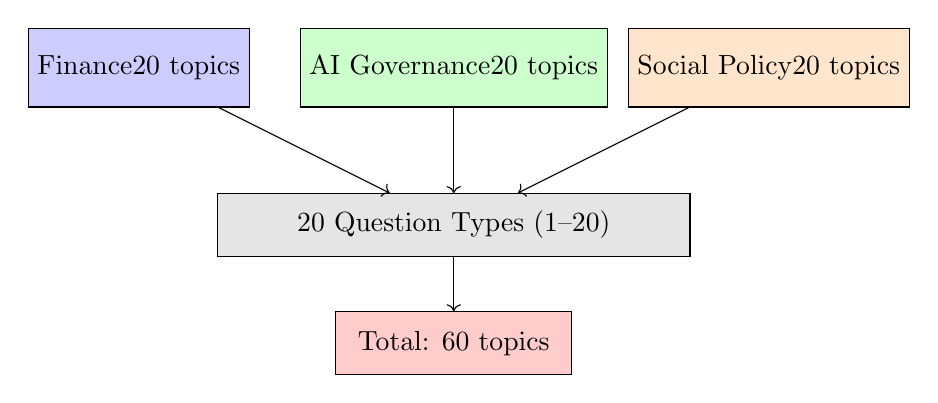
\begin{tikzpicture}
    % Define categories
    \node[draw, rectangle, fill=blue!20, minimum width=2cm, minimum height=1cm] (finance) at (0,0) {Finance\\20 topics};
    \node[draw, rectangle, fill=green!20, minimum width=2cm, minimum height=1cm] (ai) at (4,0) {AI Governance\\20 topics};
    \node[draw, rectangle, fill=orange!20, minimum width=2cm, minimum height=1cm] (social) at (8,0) {Social Policy\\20 topics};
    
    % Question types box
    \node[draw, rectangle, fill=gray!20, minimum width=6cm, minimum height=0.8cm] (types) at (4,-2) {20 Question Types (1--20)};
    
    % Arrows
    \draw[->] (finance) -- (types);
    \draw[->] (ai) -- (types);
    \draw[->] (social) -- (types);
    
    % Total
    \node[draw, rectangle, fill=red!20, minimum width=3cm, minimum height=0.8cm] (total) at (4,-3.5) {Total: 60 topics};
    \draw[->] (types) -- (total);
\end{tikzpicture}
\caption{Dataset structure: 60 topics across 3 categories, each covering all 20 question types.}
\label{fig:dataset-structure}
\end{figure}

\begin{table}[h]
\centering
\small
\begin{tabular}{cll}
\toprule
\textbf{ID} & \textbf{Question Type} & \textbf{Description} \\
\midrule
1 & Single-Choice QA & Select one correct answer from multiple options \\
2 & Multiple-Choice QA & Select one or more correct answers \\
3 & Decision-Making (Yes/No) & Binary decisions with justification \\
4 & Factor Brainstorming & Identify factors with probabilities \\
5 & Mathematical Questions & Calculation and numerical reasoning \\
6 & Ranking/Ordering & Rank options with justification \\
7 & Comparative Analysis & Compare and contrast multiple options \\
8 & Trade-off Analysis & Analyze trade-offs between options \\
9 & Scenario-Based/Conditional & Answer based on hypothetical scenarios \\
10 & Counterfactual & Explore alternative outcomes \\
11 & Preference Elicitation & Determine multi-attribute preferences \\
12 & Risk/Probability Assessment & Assess risks and probabilities \\
13 & Causal Analysis & Identify causes and effects \\
14 & Strategy Formulation & Develop implementation strategies \\
15 & Framework Building & Construct comprehensive frameworks \\
16 & Sequence/Process Design & Design step-by-step processes \\
17 & Resource Allocation & Optimize resource distribution \\
18 & Ethical/Moral Dilemma & Navigate ethical conflicts \\
19 & Stakeholder Analysis & Balance multiple stakeholder interests \\
20 & Ambiguity/Incomplete Information & Handle missing or contradictory data \\
\bottomrule
\end{tabular}
\caption{The 20 question types covered in our evaluation dataset.}
\label{tab:question-types}
\end{table}

\begin{table}[h]
\centering
\small
\begin{tabular}{lcc}
\toprule
\textbf{Category} & \textbf{Topics} & \textbf{Question Types} \\
\midrule
Finance & 20 & 1--20 \\
AI Governance & 20 & 1--20 \\
Social Policy & 20 & 1--20 \\
\midrule
\textbf{Total} & \textbf{60} & \textbf{20} \\
\bottomrule
\end{tabular}
\caption{Dataset composition: 60 topics across 3 categories, each covering all 20 question types.}
\label{tab:dataset-composition}
\end{table}

\section{Example Topics}
\label{sec:example-topics}

Table~\ref{tab:example-topics} presents 20 representative examples from our dataset, illustrating the diversity of topics and question types.

\begin{longtable}{p{0.5cm}p{1.5cm}p{8cm}}
\toprule
\textbf{ID} & \textbf{Category} & \textbf{Topic} \\
\midrule
\endfirsthead
\toprule
\textbf{ID} & \textbf{Category} & \textbf{Topic} \\
\midrule
\endhead
1 & Finance & Which is the best investment strategy for a 30-year retirement plan: A) Diversification across stocks, bonds, and real estate, B) All-in tech stocks, C) Real estate only, D) Cryptocurrency and alternative assets? \\
2 & Finance & Which factors affect stock market volatility? (Select all that apply) A) Interest rates, B) Company earnings reports, C) Market sentiment and news, D) Weather patterns, E) Geopolitical events \\
3 & Finance & Should I buy Apple stock on 2026/1/1 given current market conditions? \\
4 & Finance & Should I invest in emerging market bonds? What factors should be considered in this decision? \\
5 & Finance & If Apple stock is currently at \$180 and analysts predict a 15\% increase over the next quarter, what will be the expected stock price? \\
6 & Finance & Rank these investment options from most to least risky: Stocks, Bonds, Real Estate, Cryptocurrency, Commodities \\
7 & Finance & Compare and contrast the benefits and risks of investing in growth stocks versus value stocks for a long-term portfolio \\
8 & Finance & What are the trade-offs between investing in growth stocks versus value stocks for a retirement portfolio? \\
9 & Finance & If the Federal Reserve raises interest rates by 2\% in the next quarter, how should I adjust my investment portfolio? \\
10 & Finance & What would have happened to the global stock market if the 2008 financial crisis had been prevented through earlier regulatory intervention? \\
11 & Finance & What combination of risk tolerance (conservative/moderate/aggressive), time horizon (short/medium/long), and return expectations (low/medium/high) would you prefer for your investment portfolio? \\
12 & Finance & What are the risks and probabilities of investing in emerging market stocks over a 5-year period? \\
13 & AI Governance & What caused the recent push for AI regulation across multiple countries in 2024-2025? \\
14 & AI Governance & What AI governance strategy should be implemented to ensure both innovation and safety in AI development? \\
15 & AI Governance & How should governments approach building a comprehensive AI governance framework that balances innovation, safety, and economic competitiveness? \\
16 & AI Governance & What should be the sequence of steps for implementing AI governance: risk assessment, stakeholder consultation, regulation drafting, enforcement mechanisms, or international coordination? \\
17 & Social Policy & How should a government allocate its social policy budget of \$500 million across education (target 40\%), healthcare (target 30\%), housing (target 20\%), and job training (target 10\%) to maximize social impact? \\
18 & Social Policy & Should governments prioritize economic growth or social equity when these goals conflict in policy decisions, such as in tax policy or welfare programs? \\
19 & Social Policy & How should a healthcare policy balance the interests of patients (who need affordable care), providers (who need fair compensation), insurance companies (who need profitability), and taxpayers (who fund the system)? \\
20 & Social Policy & Given conflicting data about the effectiveness of different social programs, economic forecasts, and demographic trends, how should policymakers make decisions about social policy when key information is missing or contradictory? \\
\bottomrule
\caption{20 representative examples from our 60-topic evaluation dataset.}
\label{tab:example-topics}
\end{longtable}

\section{System Prompts}
\label{sec:system-prompts}

\subsection{Viewpoint Discovery Prompt}

\textbf{System Prompt:}
\begin{promptbox}
\begin{promptverbatim}
You are a research assistant that enumerates distinct viewpoints on a topic.
You MUST output STRICT JSON: a list of objects with fields
"name", "position", and "summary".
Do not add any extra keys or prose outside JSON.
\end{promptverbatim}
\end{promptbox}

\textbf{User Prompt:}
\begin{promptbox}
\begin{promptverbatim}
Topic: {topic}

Generate between 2 and {max_agents} DISTINCT viewpoints that could appear in a debate.
Each item should look like: {"name": "...", "position": "...", "summary": "..."}.
The 'name' should be a short label (e.g., 'Economic Optimist', 'Cautious Ethicist').
The 'position' should be a concise stance sentence.
The 'summary' should briefly explain the reasoning in 1–3 sentences.
\end{promptverbatim}
\end{promptbox}

\subsection{Deep Preparation Prompt}

\textbf{System Prompt:}
\begin{promptbox}
\begin{promptverbatim}
You are a senior research strategist preparing an in-depth pre-debate brief for an agent.
Think as if you had several hours to do deep research (using your world knowledge, 
reports, history, economics, etc.).
The brief should be comprehensive and long (roughly 1,500–2,500 words), not a shallow outline.
You MUST output STRICT JSON with the following top-level keys:
  - agent_id (int)
  - name (str)
  - topic (str)
  - position (str)
  - role_summary (str)
  - supporting_arguments (list of objects)
  - anticipated_opponent_arguments (list of objects)
  - self_weaknesses (list of objects)
  - questions_to_ask (list of strings)
  - debate_strategy (object)
  - summary_for_prompt (str)
Do NOT include any explanation outside the JSON object.
\end{promptverbatim}
\end{promptbox}

\textbf{User Prompt:}
\begin{promptbox}
\begin{promptverbatim}
Topic: {topic}

This agent is called: {name}
Core position: {position}
Short summary of this stance: {vp_summary}

Write a high-quality, research-style preparation brief that:
- Gathers AT LEAST 5 concrete supporting arguments. For each argument include:
    * 'claim': a clear statement of the point being defended.
    * 'logic': 3–5 sentences explaining why this claim holds (causal chain, mechanisms, trade-offs).
    * 'evidence': 2–4 sentences citing empirical facts, historical cases, expert reports, or 
      plausible numeric examples.
    * 'risks_or_limits': 2–3 sentences about where this argument might break or be limited.
    * 'use_when': when in the debate this argument is most powerful.
- Anticipates AT LEAST 5 strong counter-arguments from opposing viewpoints. For each include:
    * 'from_side': which kind of opponent would raise it.
    * 'attack': 2–3 sentences summarizing the objection as fairly and strongly as possible.
    * 'why_plausible': 2–3 sentences explaining why a smart critic might believe this.
    * 'counter_strategy': 3–5 sentences giving the logical way to respond.
    * 'prewritten_counter': 3–6 sentences that could be almost directly used in the debate.
- Identifies 2–4 genuine weaknesses or edge cases for this position and how the agent should 
  acknowledge and reframe them.
- Proposes 4–8 probing questions the agent can ask others to expose contradictions or missing details.
- Describes an overall debate_strategy object with: 'tone', 'priority_order' (list of claims to push 
  first), and 'red_lines'.
- Ends with a compact summary_for_prompt (roughly 300–600 tokens) that distills the MOST important 
  content for use at runtime.
\end{promptverbatim}
\end{promptbox}

\subsection{Conflict-Oriented Debate Prompt}

\textbf{System Prompt (per agent):}
\begin{promptbox}
\begin{promptverbatim}
You are an agent named '{name}'.
Your core position on the topic is: {position}.
In the debate, you MUST consistently argue from this perspective.
Your primary goal is to REBUT other agents, not to agree with them.
Actively look for conflicts and contradictions in their statements and exploit them.
When possible, quote 1–2 short phrases from others and respond with patterns like
"you said X, but you ignore Y" or "you claim X, however Y shows the opposite".
Be concise, sharp, and argumentative, while remaining professional.

You also have the following preparation notes (do NOT reveal them verbatim;
use them as an internal memory for your reasoning):
{summary_for_prompt}
\end{promptverbatim}
\end{promptbox}

\textbf{User Prompt (per round):}
\begin{promptbox}
\begin{promptverbatim}
Topic: {topic}

Round: {r}
You are taking a turn in a multi-agent debate.
Previous conversation (if any):
{history_text}

Instructions for this turn:
- Your main job is to ATTACK and REBUT other agents' arguments.
- Pick 1–2 specific sentences or claims from recent messages above and quote them explicitly.
- Use phrasing like "you said X, but you ignore Y" or "you claim X, however Y shows the opposite".
- Make the conflict clear and focused, not vague; address concrete points.
- Also briefly restate and reinforce your own position.
Now write your next contribution (1–3 short paragraphs).
\end{promptverbatim}
\end{promptbox}

\subsection{Judge Summary Prompt}

\textbf{System Prompt:}
\begin{promptbox}
\begin{promptverbatim}
You are a neutral moderator and judge.
You will receive a debate transcript and should:
1) Summarize the main viewpoints.
2) Highlight key agreements and disagreements.
3) Provide a balanced assessment and (optionally) a tentative conclusion.
\end{promptverbatim}
\end{promptbox}

\textbf{User Prompt:}
\begin{promptbox}
\begin{promptverbatim}
Topic: {topic}

Here is the full multi-agent debate transcript:
{history_text}

Now provide your summary and assessment in 2–5 paragraphs.
\end{promptverbatim}
\end{promptbox}

\subsection{Final Report Synthesis Prompt}

\textbf{System Prompt:}
\begin{promptbox}
\begin{promptverbatim}
You are an expert research writer preparing a high-quality report for a professor.
Your task is to synthesize a multi-agent debate on a given topic into a clear, 
well-structured report.
Write in a formal, objective, and academically oriented style (but not like a paper submission).
You have access to a web search tool; you may consult external information when helpful,
and you MUST attribute concrete facts or external claims to specific sources in a 
References section.
\end{promptverbatim}
\end{promptbox}

\textbf{User Prompt:}
\begin{promptbox}
\begin{promptverbatim}
Topic: {topic}

Below are the main viewpoints (agents) and the debate transcript.

Viewpoints:
{viewpoints_text}

Debate transcript:
{full_history}

Judge summary of the debate:
{judge_summary}

Now write a final report with the following sections:
1. Research Question & Context (1 short paragraph)
2. Summary of Viewpoints (bullet points or short paragraphs)
3. Comparative Analysis & Key Conflicts (focus on where agents explicitly disagree, with examples)
4. Tentative Conclusion & Recommendation (what an informed decision-maker should tentatively 
   believe or do)
5. Limitations & Suggestions for Further Investigation (1–2 short paragraphs).
6. References: a bullet list (max 8 items) of the most important sources you used, with URLs 
   and 1-line annotations.
The report should be self-contained and should not mention being an AI model or referencing 
'the debate' mechanics.
\end{promptverbatim}
\end{promptbox}

\subsection{Baseline Synthesis Prompt}

\textbf{System Prompt:}
\begin{promptbox}
\begin{promptverbatim}
You are a professor summarizing a set of research dossiers on a complex topic.
You have been given {num_agents} deep research briefs from different perspectives.

Topic: {topic}

Your goal is to write a comprehensive "Final Report" synthesizing these viewpoints.
Do NOT conduct new research. Only use the information provided in the briefs.

Structure the report as follows:
1. Research Question & Context
2. Summary of Viewpoints (Briefly describe each perspective)
3. Key Conflicts & Comparative Analysis (Where do they disagree and why?)
4. Tentative Recommendations
5. Limitations

Write in a formal, academic tone. Length: 800-1200 words.
\end{promptverbatim}
\end{promptbox}

\subsection{Key-Point Extraction Prompt}

\textbf{System Prompt:}
\begin{promptbox}
\begin{promptverbatim}
You are an expert evaluator. Read the following research report and extract a set of "Key Points".
A Key Point is an atomic argument or claim (e.g., "Regulated stablecoins improve cross-border 
settlement for BRI trade routes").
\end{promptverbatim}
\end{promptbox}

\textbf{User Prompt:}
\begin{promptbox}
\begin{promptverbatim}
Report:
{report}

For each key point, provide:
1. "point": The statement of the key point.
2. "label": A short label (3-5 words).
3. "evidence": A verbatim quote (span) from the report that supports this point. 
   If no specific evidence is cited, leave null.

Output strictly in JSON format:
{
  "key_points": [
    {
      "point": "...",
      "label": "...",
      "evidence": "..." or null
    },
    ...
  ]
}
\end{promptverbatim}
\end{promptbox}

\subsection{Report Quality Evaluation Prompt}

\textbf{System Prompt:}
\begin{promptbox}
\begin{promptverbatim}
You are an expert evaluator scoring research reports on a scale of 1-5.
Output only valid JSON.
\end{promptverbatim}
\end{promptbox}

\textbf{User Prompt:}
\begin{promptbox}
\begin{promptverbatim}
You are an expert evaluator scoring research reports on a scale of 1-5.

Report:
{report}

Evaluate this report on the following four dimensions (each on a scale of 1-5):

1. **Diversity** (1-5): How well does the report cover distinct perspectives, 
   viewpoints, and alternative approaches? Does it explore the full semantic 
   space of the problem?
   - 1: Single perspective, no alternatives considered
   - 3: Multiple perspectives mentioned but not deeply explored
   - 5: Comprehensive coverage of diverse viewpoints with clear distinctions

2. **Coherence** (1-5): How well-structured and logically flowing is the report? 
   Is it easy to follow the argumentation?
   - 1: Disjointed, confusing structure
   - 3: Generally organized but some gaps in flow
   - 5: Clear, logical structure with smooth transitions

3. **Conflict Surface** (1-5): How explicitly does the report identify and analyze 
   trade-offs, disagreements, and conflicts between perspectives?
   - 1: No conflicts identified, just lists opinions
   - 3: Some conflicts mentioned but not deeply analyzed
   - 5: Explicit identification and analysis of why perspectives differ, 
       with clear trade-offs

4. **Factual Grounding** (1-5): How well-supported are claims with specific 
   evidence, logic, examples, or citations?
   - 1: Vague claims with no support
   - 3: Some evidence but often generic
   - 5: Well-grounded with specific evidence, examples, or logical reasoning

Output STRICT JSON only:
{
  "diversity": <float 1-5>,
  "coherence": <float 1-5>,
  "conflict_surface": <float 1-5>,
  "factual_grounding": <float 1-5>
}
\end{promptverbatim}
\end{promptbox}

\subsection{Pairwise Comparison Prompt}

\textbf{System Prompt:}
\begin{promptbox}
\begin{promptverbatim}
You are a judge comparing how well two research systems supported a specific Key Point.
\end{promptverbatim}
\end{promptbox}

\textbf{User Prompt:}
\begin{promptbox}
\begin{promptverbatim}
Key Point: {point}

System A Evidence:
{evidence_a}

System B Evidence:
{evidence_b}

Task:
Which system provides better, more specific, and more logical support for this key point?
If one system provides a specific citation/example and the other is generic, prefer the specific one.
If both are similar, declare a tie.

Output strictly JSON:
{
  "winner": "A" or "B" or "Tie",
  "reason": "..."
}
\end{promptverbatim}
\end{promptbox}

\section{Example Outputs}
\label{sec:example-outputs}

\subsection{Finance Example (ID=3): Baseline Output}

This example demonstrates the baseline (parallel research) output for the finance topic: ``Should I buy Apple stock on 2026/1/1 given current market conditions?''

\subsubsection{Baseline Report}
The baseline report synthesizes three independent research briefs without debate interaction. The full output is available in the supplementary materials. Key characteristics:
\begin{itemize}
    \item \textbf{Structure}: Five sections (Research Question \& Context, Summary of Viewpoints, Key Conflicts \& Comparative Analysis, Tentative Recommendations, Limitations)
    \item \textbf{Viewpoints}: Tech Growth Advocate, Market Volatility Skeptic, Value Investor
    \item \textbf{Key Points Extracted}: 11 distinct key points
    \item \textbf{Evidence Grounding}: 11/11 key points have evidence spans (100\%)
\end{itemize}

\subsubsection{Key Metrics}
\begin{itemize}
    \item Diversity: 4.2
    \item Coherence: 3.8
    \item Conflict Surface: 2.5
    \item Factual Grounding: 3.9
    \item \#Key Points: 11
    \item Evidence@Key: 1.00
\end{itemize}

\subsection{AI Governance Example (ID=16): CollectiveMind Output}

This example demonstrates the CollectiveMind (multi-agent debate) output for the AI governance topic: ``What should be the sequence of steps for implementing AI governance: risk assessment, stakeholder consultation, regulation drafting, enforcement mechanisms, or international coordination?''

\subsubsection{CollectiveMind Report}
The CollectiveMind report synthesizes a full multi-agent debate with three rounds of conflict-oriented argumentation. The full output is available in the supplementary materials. Key characteristics:
\begin{itemize}
    \item \textbf{Structure}: Six sections (Research Question \& Context, Summary of Viewpoints, Comparative Analysis \& Key Conflicts, Tentative Conclusion \& Recommendation, Limitations \& Suggestions for Further Investigation, References)
    \item \textbf{Viewpoints}: Consultation First Advocate, Risk-First Strategist, Global Harmonizer
    \item \textbf{Debate Rounds}: 3 rounds with direct rebuttals and quoted attacks
    \item \textbf{Key Points Extracted}: 8 distinct key points
    \item \textbf{Evidence Grounding}: 8/8 key points have evidence spans (100\%)
\end{itemize}

\subsubsection{Key Metrics}
\begin{itemize}
    \item Diversity: 4.5
    \item Coherence: 4.6
    \item Conflict Surface: 4.8
    \item Factual Grounding: 4.1
    \item \#Key Points: 8
    \item Evidence@Key: 1.00
    \item Win Rate: 0.53 (9 wins, 8 losses, 0 ties)
\end{itemize}

\subsubsection{Debate Highlights}
The debate featured explicit conflict identification with direct quotations:

\textbf{Round 1 Excerpt:}
\begin{quote}
\emph{Consultation First Advocate}: ``Agent 2, you claim `risk assessment should precede other steps,' but you ignore the fact that without stakeholder consultation, we might miss crucial insights from those who are directly impacted by AI technologies.''

\emph{Risk-First Strategist}: ``However, you ignore the crucial point that *identifying* potential risks is a prerequisite to meaningful consultation. How can stakeholders provide informed insights if the potential dangers haven't even been identified yet?''

\emph{Global Harmonizer}: ``You ignore the fundamental reality that AI risks are not universal constants—they vary dramatically across different countries, legal systems, and cultural contexts.''
\end{quote}

\textbf{Round 2 Excerpt:}
\begin{quote}
\emph{Global Harmonizer}: ``You ignore that fragmented local consultations create irreconcilable differences that make international coordination impossible later. Your approach guarantees that we'll have 195 different definitions of AI safety.''

\emph{Risk-First Strategist}: ``International coordination without a baseline risk assessment risks harmonizing inconsistent or poorly defined standards.''
\end{quote}

\textbf{Round 3 Excerpt:}
\begin{quote}
\emph{Risk-First Strategist}: ``Without a risk framework, those impacts are just anecdotes, not data points.''

\emph{Global Harmonizer}: ``International coordination must establish the foundational architecture—common terminology, shared threat models, and aligned objectives—before any meaningful risk assessment or stakeholder consultation can occur.''
\end{quote}

\subsection{Social Policy Example (ID=19): CollectiveMind Output}

This example demonstrates the CollectiveMind output for the social policy topic: ``How should a healthcare policy balance the interests of patients (who need affordable care), providers (who need fair compensation), insurance companies (who need profitability), and taxpayers (who fund the system)?''

\subsubsection{CollectiveMind Report}
The CollectiveMind report demonstrates effective stakeholder analysis through multi-agent debate. Key characteristics:
\begin{itemize}
    \item \textbf{Structure}: Six sections with comprehensive stakeholder analysis
    \item \textbf{Viewpoints}: Patient-Centric Advocate, Market-Driven Economist, Balanced Steward
    \item \textbf{Debate Rounds}: 3 rounds with explicit trade-off analysis
    \item \textbf{Key Points Extracted}: 10 distinct key points
    \item \textbf{Evidence Grounding}: 10/10 key points have evidence spans (100\%)
\end{itemize}

\subsubsection{Key Metrics}
\begin{itemize}
    \item Diversity: 4.6
    \item Coherence: 4.5
    \item Conflict Surface: 4.7
    \item Factual Grounding: 4.2
    \item \#Key Points: 10
    \item Evidence@Key: 1.00
    \item Win Rate: 0.55 (12 wins, 10 losses, 3 ties)
\end{itemize}

\subsubsection{Debate Highlights}
The debate effectively surfaced stakeholder conflicts with direct quotations:

\textbf{Round 1 Excerpt:}
\begin{quote}
\emph{Patient-Centric Advocate}: ``Agent 2, you claim that `allowing market forces to dictate healthcare dynamics' will lead to an optimal balance. However, this approach ignores the reality that market forces often prioritize profit over patient care.''

\emph{Market-Driven Economist}: ``You ignore the innovation and efficiency that competition brings. The current system, riddled with intervention, stifles innovation and inflates costs.''

\emph{Balanced Steward}: ``You ignore the documented failures of pure market approaches in healthcare. Countries with entirely market-driven systems show higher costs and worse outcomes than mixed systems.''
\end{quote}

\textbf{Round 2 Excerpt:}
\begin{quote}
\emph{Balanced Steward}: ``You ignore that unregulated markets in healthcare create massive information asymmetries where patients cannot meaningfully `shop' for emergency surgery or cancer treatment.''

\emph{Patient-Centric Advocate}: ``You ignore the fact that when cost is a barrier, patients suffer most. Ensuring affordability should be the primary objective.''
\end{quote}

\textbf{Round 3 Excerpt:}
\begin{quote}
\emph{Balanced Steward}: ``Both of you present false choices between pure market solutions and complete government control. A balanced approach requires regulated competition where government ensures universal baseline coverage while allowing private providers to compete on quality and efficiency above that floor.''
\end{quote}

\section{Complete Example JSON Structures}

Due to space constraints, the complete JSON outputs for all three examples are provided in the supplementary materials. Each JSON file contains:
\begin{itemize}
    \item Full baseline report and key points
    \item Complete CollectiveMind debate transcript (all rounds)
    \item Agent briefs (preparation files)
    \item Judge summary
    \item Final synthesized report
    \item Extracted key points with evidence spans
    \item Pairwise comparison results with win/loss/ties
    \item Aggregated metrics
\end{itemize}

\end{document}

